%!TEX root = ../main.tex
\section{Augmenting path algorithms}
\subsection{Introduction}
The idea behind the augmenting path algorithms is as follows : 
As long as there is a path from the source to the sink, we send flow along this path. And so on until there is no more path from the source to the sink. \newline

An available path from the source to the sink is called \textit{augmenting path} and to find it, we use the \textit{residual graph}. A \textit{residual graph} is a double oriented graph with the available capacities. For instance here is a graph with its \textit{residual graph}: \newline

\begin{figure}[!h]
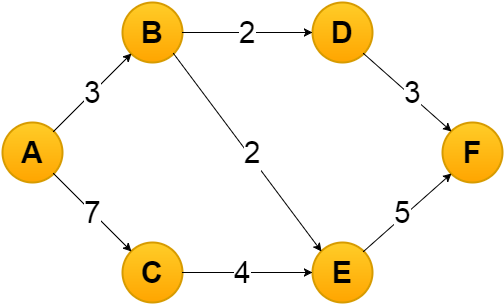
\includegraphics[width=7.5cm,height=4.5cm]{images/graph.png}\hfill
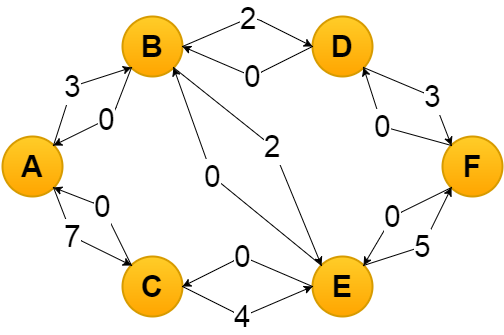
\includegraphics[width=7.5cm,height=4.5cm]{images/residualgraph.png}
\caption{Graph with its residual graph}
\end{figure}


When an \textit{augmenting path} is found, we send a flow equivalent to the minimum capacity of the edges of this path. We update the \textit{residual graph} and then we look for a new augmenting path. \newline

Here is the \textit{residual graph} after sending 4 units of flow through the \textit{augmenting path} A-C-E-F : \newline

\begin{center}
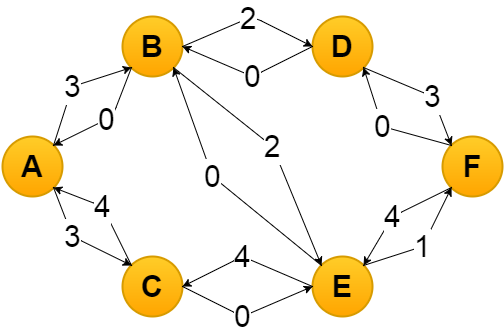
\includegraphics[width=7.5cm,height=4.5cm]{images/residualgraph2.png}
\captionof{figure}{Residual graph}
\end{center}

The pseudo-code of the augmenting path algorithm is given here :

\begin{algorithm}[h]

 Look for an augmenting path\;
 \While{There is an augmenting path}{
  Send flow through this path\;
  Update the residual graph\;
  Look for an new augmenting path\;
 }
\end{algorithm}

\subsection{Ford-Fulkerson vs Edmonds-Karp}
Je cause de la différence entre FF et EK

\subsection{Complexities}
Petite intro pour dire que c'est polynomial
\subsubsection{Ford-Fulkerson}

\subsubsection{Edmonds-Karp}
Il faut démontrer que la complexité grand O est pas possible?

\section{Pre-flow algorithms}
